\subsection{Grading based on Inlinks and Outlinks} % eller: Grading based on inlink and outlinks 
Our first assumption is that categories with high a inlink number can be reached from categories with different topics. An example of a category with a high inlink number is  \emph{World War II}. This category can be reached from 87 different categories (see figure \ref{fig:high_inlink_number}). 

%great rift valley: 5, 31
%world war ii
%87
%['1940s conflicts', 'wars involving saudi arabia', 'wars involving austria', 'wars involving estonia', 'wars involving costa rica', 'wars involving the republic of china', 'wars involving panama', 'wars involving peru', 'wars involving vietnam', 'the world wars', 'wars involving the netherlands', 'wars involving syria', 'wars involving ethiopia', 'wars involving iraq', 'wars involving norway', 'wars involving nicaragua', 'conflicts in 1941', 'conflicts in 1940', 'conflicts in 1943', 'conflicts in 1942', 'conflicts in 1945', 'conflicts in 1944', 'wars involving liberia', 'wars involving ukraine', 'wars involving egypt', 'wars involving nepal', 'wars involving bolivia', 'wars involving san marino', 'wars involving albania', 'wars involving the philippines', 'wars involving iran', 'commons category wikidata tracking categories', 'wars involving italy', '1930s conflicts', 'wars involving the united states', 'wars involving british india', 'wars involving poland', 'wars involving el salvador', 'global conflicts', 'wars involving the soviet union', 'wars involving luxembourg', 'wars involving venezuela', 'wars involving new zealand', 'wars involving brazil', 'wars involving mexico', '20th-century conflicts', 'wars involving cuba', 'wars involving france', 'wars involving hungary', 'wars involving indonesia', 'wars involving greece', 'wars involving colombia', 'wars involving argentina', 'wars involving ecuador', 'wars involving czechoslovakia', 'modern europe', 'wars involving lebanon', 'wars involving turkey', 'wars involving haiti', 'wars involving chile', 'wars involving thailand', 'wars involving yugoslavia', 'wars involving korea', 'wars involving lithuania', 'wars involving mongolia', 'wars involving cambodia', 'wars involving the dominican republic', 'wars involving bulgaria', 'wars involving belgium', 'wars involving japan', 'wars involving laos', 'wars involving finland', 'wars involving australia', 'wars involving canada', 'wars involving paraguay', 'wars involving uruguay', 'wars involving romania', 'wars involving belarus', 'wars involving guatemala', 'wars involving the united kingdom', 'conflicts in 1939', 'wars involving burma', 'wikipedia category maintenance', 'wars involving south africa', 'wars involving honduras', 'wars involving denmark', 'wars involving germany']

\begin{figure}[h]
\centering
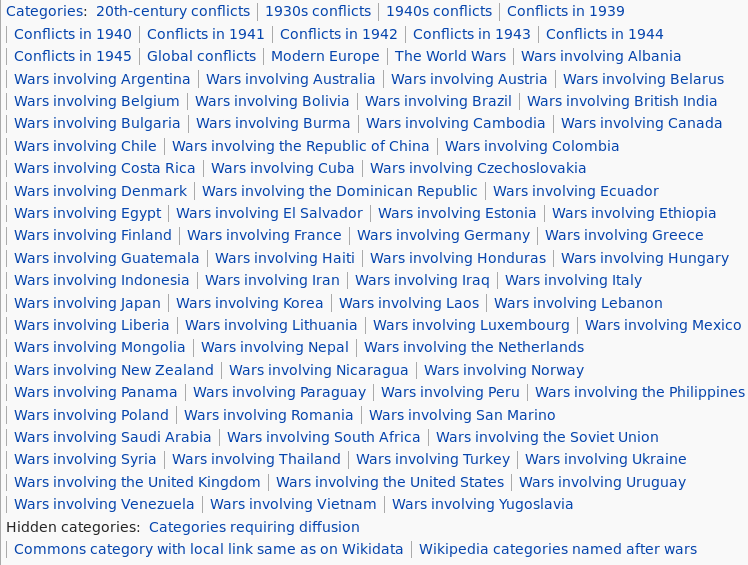
\includegraphics[width=\textwidth]{Chapters/Implementation/Grading/high_inlink_number}
\caption[Example of category with high \emph{inlink number}]{All categories linking to the category \emph{World War II}. This is an example of a category with high inlink number.}
\label{fig:high_inlink_number}
\end{figure}


\begin{comment}
\begin{figure}[h]
\centering
\begin{lstlisting}
ole-johan dahl:
*politics/political activism/leadership/management/quality/software quality/formal methods/formal methods people
\end{lstlisting}
\caption{Example of how \emph{politics} can reach the article about \emph{Ole-Johan Dahl}}
\label{fig:politicstosoftware}
\end{figure}
\end{comment}
%quality: 9, 3
%management: 31, 5
The next assumption is that categories with a high outlink number are more likely to reach categories not relevant since they can reach far in all the subcategories' directions. Figure \ref{fig:high_outlink_number} illustrates number of subcategories found for the category with highest outlink number, which is the category \emph{Albums by artist} and a outlink number of 17 393. 

%Figure \ref{fig:politicstosoftware} shows how the Wikipedia article about \emph{Ole-Johan Dahl} can be reached from the category \emph{politics}. One of the categories with a high \emph{outlink} is the category \emph{management}, which has \emph{outlink} as 31 and hence be reached many categories. 

\begin{figure}[h]
\centering
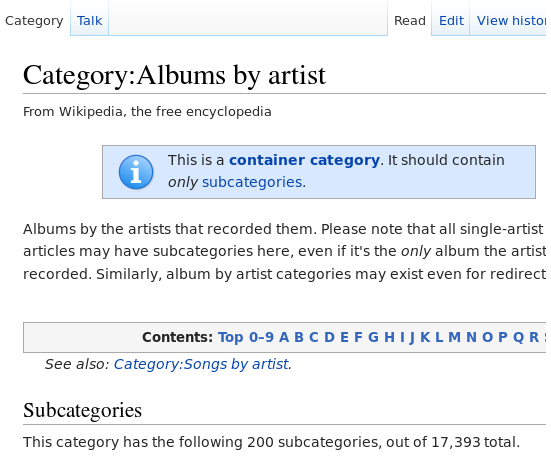
\includegraphics[width=0.7\textwidth]{Chapters/Implementation/Grading/high_outlink_number}
\caption[Example of category with high \emph{outlink number}]{The category \emph{Albums by artist} is an example of category with high outlink number. }
\label{fig:high_outlink_number}
\end{figure}


%\subsubsection{Grading based on Inlinks and Outlinks}
These assumption combined are the foundation of grading based on inlink and oulink numbers. Categories frequently reached should obtain a lower score than categories rarely reached. We need some way of deciding whether an inlink number is high for each category. This can be done by comparing the inlink number with the average inlink number, and similarly for outlink number and the average outlink number. 

%Thus, our first approach was to find the \emph{inlink} and \emph{outlink} of all categories in the structure. 

The average inlink and outlink numbers are found by summarizing all inlink numbers and outlink number respecitvely, and dividing the result on number of categories. Table \ref{tab:avginlinkoutlink} shows the tesults found. 

%numbers had to be compared with the average number of \emph{inlink} and \emph{outlink} to know whether the number is high or low (see Table \ref{tab:avginlinkoutlink}). 


\begin{table}[ht]
\centering
\renewcommand{\arraystretch}{1.25}
\begin{tabularx}{\textwidth}{c |c}
\textbf{Average \emph{inlink number}} & \textbf{Average \emph{outlink number}}\\ \hline
 5 & 2 \\
\end{tabularx}
\\[10pt]
\caption{Average inlink number and outlink number for all categories.}
\label{tab:avginlinkoutlink}
\end{table}
The score for each category was found by comparing its inlink number and outlink number by the average inlink and outlink number, i.e. 

\begin{equation} \label{eq:scoreinout}
Score_{C} = \frac{inlink_{c} + outlink_{c}}{\bar{C_{in}} + \bar{C_{out}}}
\end{equation}
where $\bar{C_{in}}$ is the average \emph{inlink} and $\bar{C_{out}}$ is the average \emph{outlink}.

%The scoring from formula \ref{eq:scoreinout} means that paths with categories rarely visited will be favoured, hence given a lower score. 

\subsubsection{Evaluation of the scores}
None of the categories can have a score of 0 since all Wikipedia categories are connected to at least one other category \footnote{We mentioned in challenges (Introduction, encoding)that some of our connections were broken. This does not affect the scoring of the categories, since the inlink and outlink numbers are preserved for all categories. }. The lowest score found was 0.376010, which was given to all categories with only one parent category and with none subcategories. This was a total of 104 471 categories.  The category with the highest score is the category \emph{Albums by Artist}, which is the category with most subcategories (17 393), hence a score of $6 512.120784$. The range of the scores is \emph{<0.376010, 6 512.120784>}, which means that all scores is within this range. 

Figure \ref{fig:scorevalue} shows how many categories are found for each of the possible score values. The figure shows that there are many categories with low score values, while there are only a few categories for higher score values. The categories with high score value will have a high impact on the article path, paths containing these categories will have a lower probability of be considered relevant. 


\begin{figure}[h]
\centering
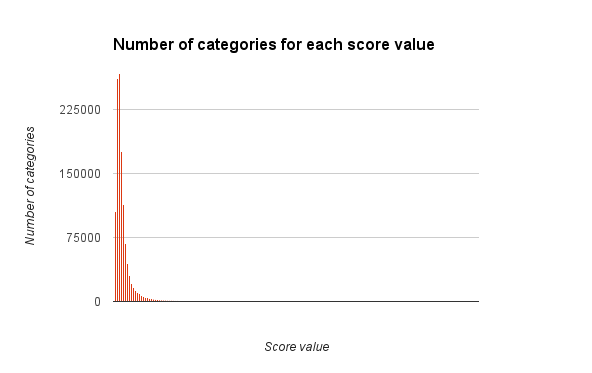
\includegraphics[width=\textwidth]{Chapters/Implementation/Grading/Inlinkoutlink_scorevalue_numberofcategories}
\caption{Number of categories for each possible score value}
\label{fig:scorevalue}
\end{figure}

%This means that the score for all categories are between 0.376010 and 6512.120784.

%This means that the scores for all categories are in the range of 0 and

%Maxgrade: 6512.120784 (albums by artist)
%Mingrade: 0.376010 (user bho-4)
\subsection{Problems with the simplified grader}
Since it is desirable with the lowest score as possible, the first problem encountered was that the program favoured short paths. 

\begin{figure}
\centering
\begin{lstlisting}
argentines of serb descent:
* society/ethnicity/ethnicity stubs/ (34.592939)
* culture/ethnicity/ethnicity stubs/ (29.704807)
* humans/ethnic groups/ethnology/ethnicity stubs/ (27.824755)
\end{lstlisting}
\caption{Caption}
\label{fig:my_label}
\end{figure}

This is both correct and wrong at the same time. It is desirable to find short paths, but there should be some punishment if the path is too short?

\begin{comment}
Problem med Alexander Huges: han er fotballspiller og dette kommer ikke så godt fra. 

asd.,kas.kdfj
\end{comment}


\begin{figure}[h]
\centering
\begin{lstlisting}
alexander hughes:
*health/health by city/health in edinburgh/sport in edinburgh/sports teams in edinburgh/football clubs in edinburgh/heart of midlothian f.c./heart of midlothian f.c. players (37.22501)
*nature/life/births by year/year of birth missing (28.576777)
*people/people categories by parameter/people by time/births by year/year of birth missing (28.200766)
\end{lstlisting}

\caption{Caption}
\label{fig:alexanderhughes}
\end{figure}
